The TEM method was originlly introduced for mining applications~\parencite{chandraTimeDomainElectromagnetic2016} 
and was since adopted to other fields like groundwater, 
and geothermal exploration~\parencite{chandraTimeDomainElectromagnetic2016, everettElectromagneticInduction2013}.
The transient electromagnetic (TEM) or altenatively time-domain electromagnetic (TDEM) method was
proposed by \textcite{obukhovFieldsHorizontalElectric1968} and has been intensively developed 
in the 1980s~\parencite{christiansenTransientElectromagneticMethod2006}.

\subsection{Transient Electromagnetic Method}\label{subsec:tem-method}
For the TEM method a pulse of current is transmitted through a ungrounded transmitter loop 
generating a primary magnetic field~\parencite{chandraTimeDomainElectromagnetic2016,christiansenTransientElectromagneticMethod2006}.
When the current is turned off, the decay of the primary field induces 
secondary currents (eddy currents) in the ground,
which produce a secondary magnetic field~\parencite{chandraTimeDomainElectromagnetic2016,christiansenTransientElectromagneticMethod2006}.
This is governed by the Maxwell equations, which state that a changing electrical field 
induces a magnetic field, and vice versa~\parencite{christiansenTransientElectromagneticMethod2006}.
An electromagnetic (EM) wave propagating through the subsurface, 
is attenuated by the electrical properties of the materials it encounters~\parencite{christiansenTransientElectromagneticMethod2006,everettElectromagneticInduction2013}.
The strength of the secondary magnetic field depends on the conductivity of the material the EM wave propagates through 
and by measuring this field over time using a receiver loop, 
information about the subsurface can be obtained~\parencite{christiansenTransientElectromagneticMethod2006,chandraTimeDomainElectromagnetic2016}.
Data is recorded in specific time-windows (gates), 
which are usually logarithmically spaced to increase signal-to-noise (S/N) ration in later times, 
which is called log-gating~\parencite{christiansenTransientElectromagneticMethod2006}.
Such a decay curve of the secondary magnetic field over time is called a ``transient'', 
with an numerically modelled example shown in \cref{fig:typical_sounding}(b).

\begin{figure*}[ht]
    \centering
    \includegraphics[width=0.7\linewidth]{data/example_modelled/example_response.png}
    \caption{Numerically modelled typical TEM response with the used subsurface model (a), 
    the signal (b), and the apparent resistivity (c).}
    \label{fig:typical_sounding}
\end{figure*}

By analysing the decay characteristics of a transient, it is possible to infer the conductivity structure of the subsurface,
because with passing time the EM wave propagates deeper into the subsurface 
and thus later time gates are linked to information about deeper layers~\parencite{christiansenTransientElectromagneticMethod2006}.
The depth of investigation (DOI) is limited by the electrical conductivity of the subsurface,
because a EM wave attenuates stronger within a conductive layer~\parencite{everettElectromagneticInduction2013}.
For this reason the TEM method is commonly deployed to investigate conductive layers such as sea water intrusions, and
clay layers confining aquifers~\parencite{chandraTimeDomainElectromagnetic2016}.

Every geophysical measurement includes uncertainty
and a single transient is usually significantly influenced by background noise~\parencite{christiansenTransientElectromagneticMethod2006,everettElectromagneticInduction2013}.
To increase the S/N ratio of a TEM sounding measurents are repeated 
and the resulting transients are combined, which is called ``stacking''~\parencite{christiansenTransientElectromagneticMethod2006}.
Commonly between $1000$ and $10000$ transients are stacked into one sounding~\parencite{aignerFlexibleSingleLoop2021} 
and when utilising a log-gating technique the S/N ratio is improved by the factor $\sqrt{\text{N}}$ where $\text{N}$ is the amount of 
measurements per stack~\parencite{christiansenTransientElectromagneticMethod2006}.

A first evaluation of the data collected can be to convert the transient from voltage readings to apparent elctrical resistivity ($\rho_\text{a}$), 
which equals to the weighted mean of the resistivities of the layers in which the currents were induced~\parencite{siemonElectromagneticMethodsFrequency2009}.
If the EM wave travels through a half-space, the late-time apparent resistivities is given by
\begin{equation}
    \rho_a = \frac{1}{\pi} \left( \frac{M}{20 \cdot \frac{\partial b_z}{\partial t}} \right)^{\frac{2}{3}} \left( \frac{\mu_0}{t} \right)^{\frac{5}{3}}
    \label{eq:apparent_resistivity}
\end{equation}
where $M$ is the magnetic moment, $\frac{\partial b_z}{\partial t}$ is the signal measured by the receiver coil,
$\mu_0$ is the magnetic permeability of free space and $t$ is the time~\parencite{fittermanTransientElectromagneticSounding1986}.
The magnetic moment is the product of the number of turns, the area, and the current in the transmitter loop.
\cref{fig:typical_sounding} shows a numerically modelled example, where (a) is the one dimensional model of the layered half-space,
(b) is the modelled decay of the secondary magnetic field, and (c) shows the converted apparent resistivity.
\cref{fig:typical_sounding} shows that in a layered half-space the resistivities of the subsurface model in (a) can not be simply
infered through the apparent resistivities in (c), 
which makes the interpretation of the data necessary~\parencite{fittermanTransientElectromagneticSounding1986,christiansenTransientElectromagneticMethod2006}.
Reconstructing the resistivity distribution of the subsurface requires the solution of ill-posed problem, 
as there are many subsurface models, which can explain the measured data~\parencite{xueDevelopmentInversionMethod2020}.
Infering a subsurface model from observed data is called an inverse problem or ``inversion'' and 
will be discussed in~\cref{subsubsec:data-inversion}.
For the interpretation of TEM data -- and for the inversion in particular -- the following assumptions must to be made: 
The EM waves created by the transmitter only propagate downwards into a layered half-space and
as most inversion algorithms work with a one dimensional model, 
the subsurface is assumed to be homogeneous in the horizontal direction~\parencite{christiansenTransientElectromagneticMethod2006}.

\subsection{State of The Art}
\label{subsec:state-of-the-art}

\subfile{2.1_state_of_the_art}

\subsection{Experimental Set Up}
\label{subsec:set-up}

In order to investigate the applicability of automatically determining an optimal lambda value to TEM data, 
we conducted a field survey in October of 2024 at the Martenhofer Lacke in the Nationalpark Neusiedlersee - Seewinkel. 
Existing data available at the Geophysics Research Unit at TU Wien from May 2024 for the same location, 
but with a differing measuring configuration was also made available for this thesis, which enables a comparison between varying setups.

In frame of this thesis a python package was developed to read, filter, and invert the TEM data.
The visualisation of an L-curve as well as three techniques of automatically finding an optimal lambda were also implemented.
Namely the cubic spline method based on \textcite{lloydUseLcurveMethod1997}, 
an similar approach using the \texttt{gradient()} function from the \texttt{numpy} library, and 
the golden section search as proposed by \textcite{cultreraSimpleAlgorithmFind2020}.

\subsubsection{Measuring Device}
\label{subsubsec:device}

Field surveys were conducted with the TEM-Fast 48 HPC system by Applied Electromagnetic Research (AEMR), 
which is compact device allowing the use of a single-loop configuration~\parencite{barsukovChapter3Shallow2006,aignerFlexibleSingleLoop2021}. 
By connecting an external $12~/~24\,V$ battery a current either $1~/~4\,A$ can be put through the connected transmitter loop~\parencite{aignerFlexibleSingleLoop2021}.
It records up to 48 logarithmically spaced time gates, which results in a time range between $4 - 16000\,\mu s$~\parencite{aignerFlexibleSingleLoop2021}.
The specific number of time gates can be chosen through a time-key~\parencite{aignerFlexibleSingleLoop2021}. 
\cref{tab:time-key} shows which time-key leads to which recording time range ((Excerpt from the manual of the TEM-FAST 48 system)).
To provide an optimal signal-to-noise ratio the device automatically stacks multiple pulses~\parencite{barsukovChapter3Shallow2006}.
The number of stacks are given by the formula $P_{tot} = 13 \times n_s \times n_{as}$~\parencite{aignerFlexibleSingleLoop2021}, 
where $n_s$ ($1-20$) is the chosen stacking-key and $n_{as}$ is the number of analogue stacks depending on the chosen time-key 
and can be found in \cref{tab:time-key}.
More detailed infromation on the device can be found in the manual provided on the website \url{http://www.aemr.net/tem-fast.htm}.

\begin{table*}[!ht]
    \centering
    \caption[Time Key Parameters of the TEM-FAST Device]{Parameters relating to the time-key of the TEM-FAST 48 HPC system (Excerpt from the manual).}
    \begin{tabular}{cccc}
        \toprule
        \textbf{Key} & \textbf{Max Time ($\mu s$)} & \textbf{Time Gates} & \textbf{Analogue Stacks} \\
        \midrule
        1 & 64 & 16 & 1024\\
        2 & 128 & 20 & 512\\
        3 & 256 & 24 & 256\\
        4 & 512 & 28 & 128\\
        5 & 1024 & 32 & 64\\
        6 & 2048 & 36 & 32\\
        7 & 4096 & 40 & 16\\
        8 & 8192 & 44 & 8\\
        9 & 16384 & 48 & 4\\
        \bottomrule
    \end{tabular}
    \label{tab:time-key}
\end{table*}

\subsubsection{Field Survey}
\label{subsubsec:field-survey}

The field measurements were carried out at the Martenhofer Lacke in the \textit{Nationalpark Neusiedlersee - Seewinkel} (16° 51' 23.058'' N, 47° 45' 8.4348'' E),
which is located on the east side of the Neusiedler See, Austria.
Being part of the Seewinkel, which are intermittent alkaline soda waters, this water cycle of this lake is fueled by deep saline groundwater and evaporation 
leading to its high salinity and shallow water depth, which also varies throughout the year~\parencite{borosHowCanUnique2025}.
This location was chosen due to the lack of man-made structures in the Nationalpark, 
which reduces noise in the gathered TEM data to a minimum~\parencite{aignerSensitivityAnalysisInverted2024}.

The first survey, consisting of 45 soundings as shown in \cref{fig:may-map} with a $12.5\times12.5\,\text{m}$ square loop, was carried out on the 22nd May 2024 
and for the second survey 66 soundings, visualised in \cref{fig:oct-map} with a $6.25\times6.25\,\text{m}$ square loop were measured on 8th October 2024.
For both surveys a voltage of $24\,\text{V}$ was used and \cref{tab:sounding-parameters} shows the parameters for each sounding.
Based upon a first visual inspection of the data some soundings were marked as "anomalous" as seen in \cref{fig:may-map,fig:oct-map}.

\begin{figure}[!ht]
    \centering
    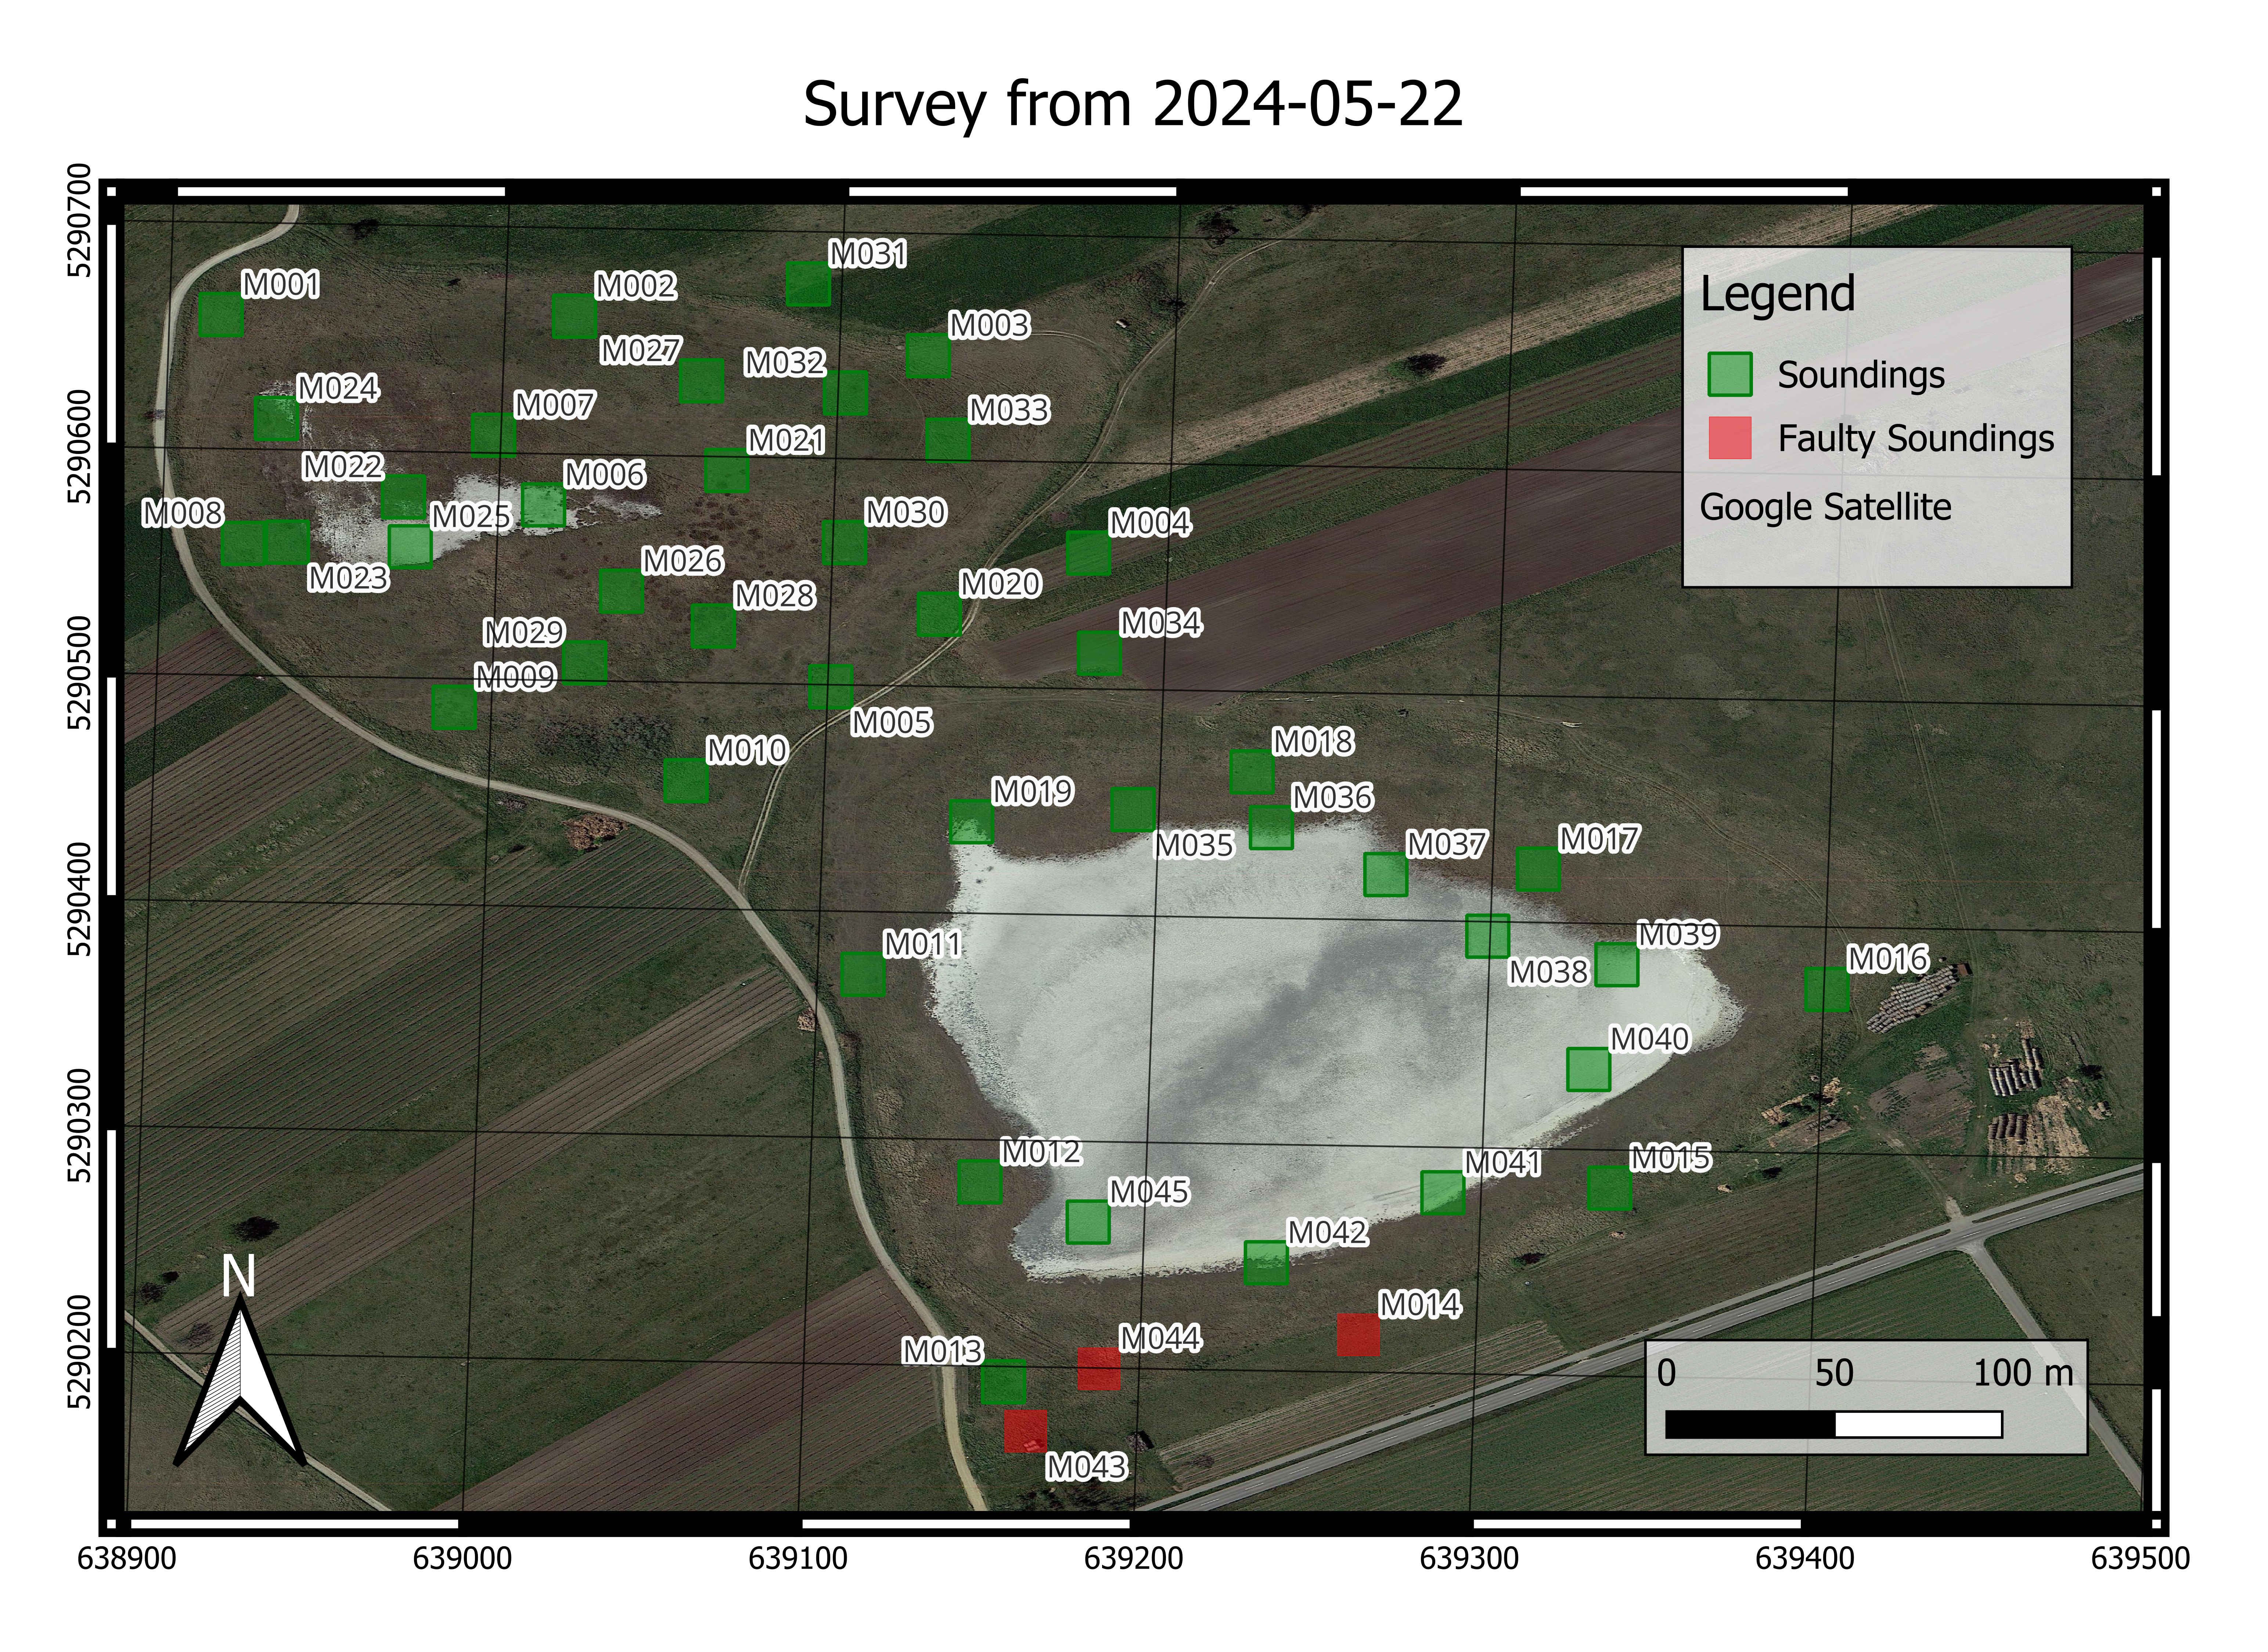
\includegraphics[width=\linewidth]{data/20240522/Survey_20240522.png}
    \caption[Map of Sounding Locations in May]{Locations of all the TEM soundings measured in the first survey (22nd May 2024), where soundings are marked as anomalies, which fell out of order in a first visual inspection.}
    \label{fig:may-map}
\end{figure}

\begin{figure}[!ht]
    \centering
    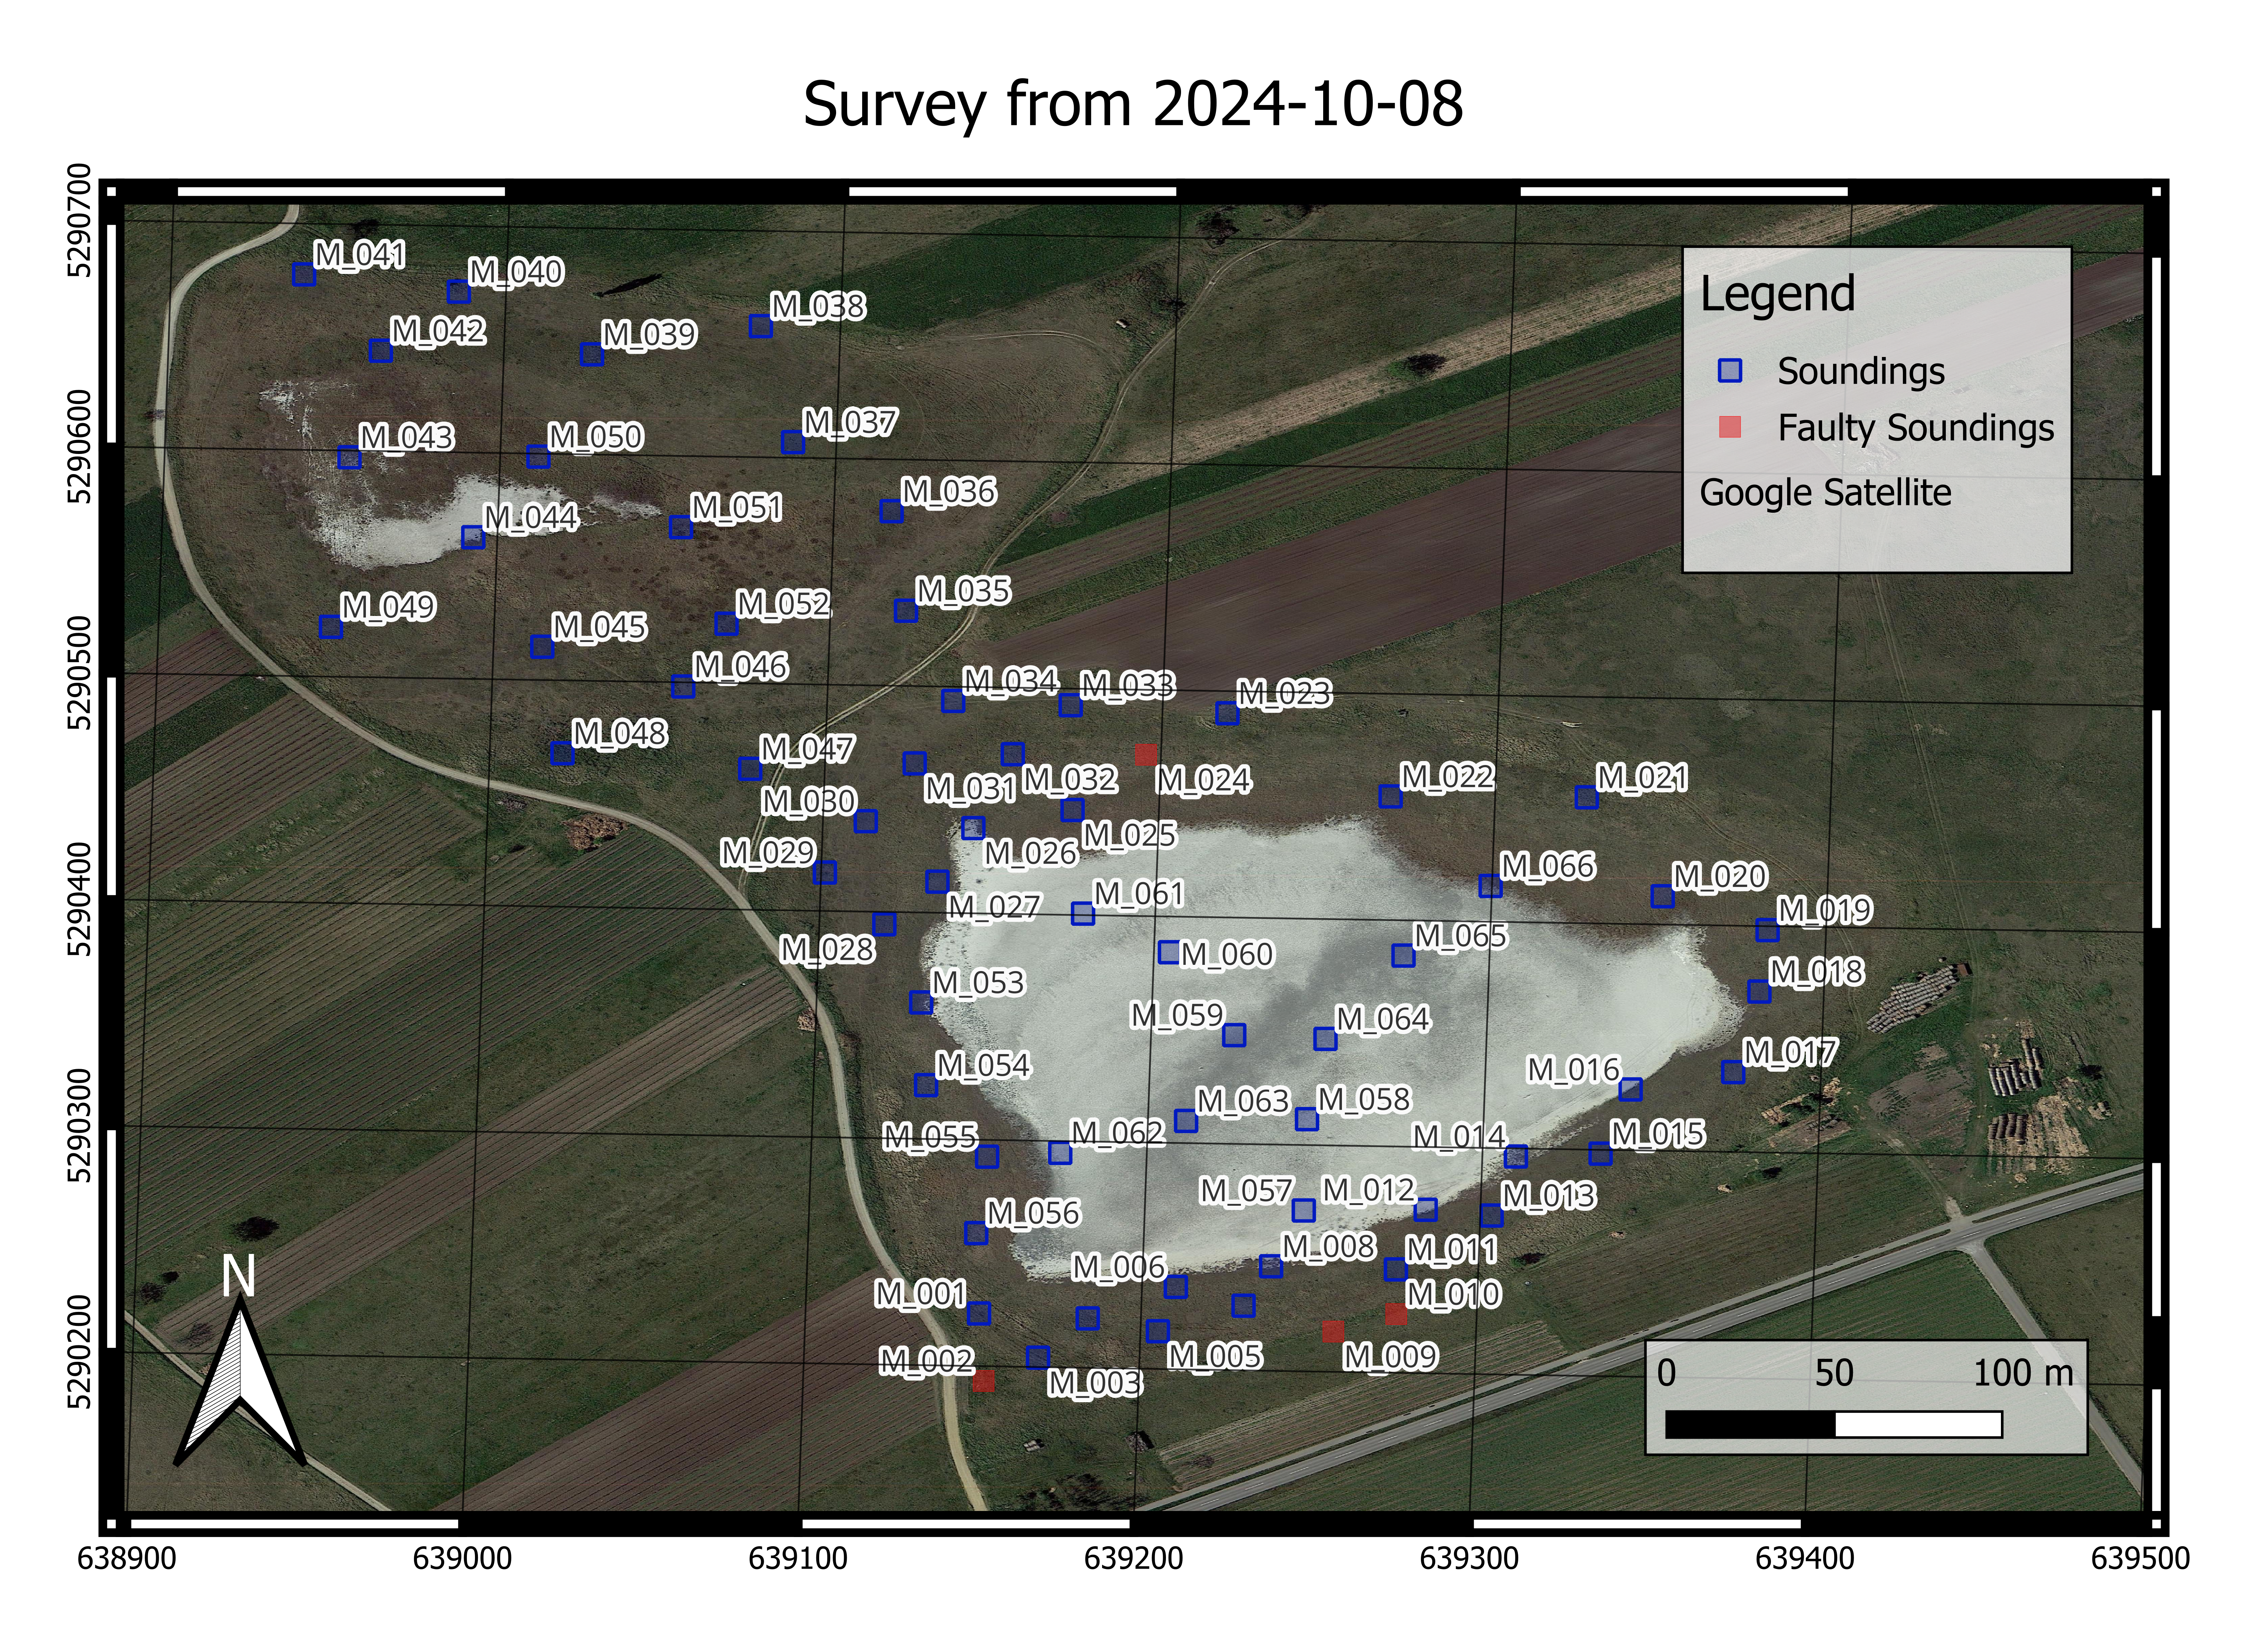
\includegraphics[width=\linewidth]{data/20241008/Survey_20241008.png}
    \caption[Map of Sounding Locations in October]{Locations of all the TEM soundings measured in the second survey (8th October 2024), where soundings are marked as anomalies, which fell out of order in a first visual inspection.}
    \label{fig:oct-map}
\end{figure}

\begin{table*}[ht]
    \centering
    \caption[Device Settings in Both Surveys]{Device settings used as well as the resulting measured time ranges and total number of pulses stacked for each sounding of both surveys.}
    \begin{tabular}{cccccc}
        \toprule
        \textbf{Sounding} & \textbf{Current} & \textbf{Time Range} & \textbf{Time Key} & \textbf{Stacking Key} & \textbf{Total Stacks} \\
        \midrule
        \textbf{22nd May 2024} \\
        $\text{M001},\,\text{M002}$ & $4.1\,\text{A}$ & $4-480\,\mu\text{s}$ & $4$ & $3$ & $4992$\\
        $\text{M003}\,-\,\text{M014}$ & $1.0\,\text{A}$ & $4-480\,\mu\text{s}$ & $4$ & $3$ & $4992$\\
        $\text{M015}\,-\,\text{M045}$ & $1.0\,\text{A}$ & $4-240\,\mu\text{s}$ & $3$ & $3$ & $9984$\\
        \textbf{8th October 2024} \\
        $\text{M001}\,-\,\text{M066}$ & $4.1\,\text{A}$ & $4-240\,\mu\text{s}$ & $3$ & $5$ & $16640$\\
        \bottomrule
    \end{tabular}
    \label{tab:sounding-parameters}
\end{table*}

\subsubsection{Python Package}
\label{subsubsec:inversion}

In order to process the gathered data, we developed a python package mainly based on open-source python libraries.
For the inversion routine we built upon the work of \textcite{aignerFlexibleSingleLoop2021}, 
which combines the electromagnetic wave modelling capabilities of \texttt{empymod}~\parencite{werthmullerOpensourceFull3D2017}
with the inversion algorithm from \texttt{PyGIMLi}~\parencite{ruckerPyGIMLiOpensourceLibrary2017}.

The capabilities of this package include the reading of TEM data, adding coordinates to each sounding, 
the filtering based upon a time intervall, and the visualisation of the raw with the filtered data.
The inversion routine requires certain starting parameters like the regularisation parameter $\lambda$, a layer distribution, 
a start model, and the relative error of the measured signal.
If not specified otherwise a homogeneous model with the median apparent resistivity of the sounding is used as the starting model
and the relative error is computed based of the error output of the measuring device.
In case of particularly noisy data it is possible to set a minimum value for the relative error (noise floor).
The noise floor can also set to entirely replace the recorded errors with a constant error vector, like \textcite{aignerFlexibleSingleLoop2021} propesed.
The relative error limits how strongly the inversion algorithm tries to fit the model to each data point to avoid fitting errors.
This inversion algorithm works with a model of the subsurface, 
where a resistivity value is assigned to a layer with a certain thickness, 
and only modifies the resistivity value of every layer while keeping the thicknesses fixed.
This makes the choice of an appropriate layer distribution (specifying the number and thicknesses of layers) vital~\parencite{welkensComparisonSubsurfaceGeophysical2025}.

The python routine described in this thesis computes and visualises an L-Curve for a TEM sounding.
For this we run the inversion for various logarithmically spaced lambda values, 
specified by the lower bound, the upper bound, and the number of values. 
For each inversion, we compute the root-mean-square (RMS) misfit of the data with the model 
as well as the roughness of the model and use these two values as the coordinates of a point
corresponding to each inversion, which should result in an L-Curve~\parencite{cultreraSimpleAlgorithmFind2020, hansenAnalysisDiscreteIllPosed1992}.

To find an optimal lambda value for the inversion we implemented three search algorithms, 
which all try to find the point (corresponding to a lambda value) with the highest curvature on the L-Curve~\parencite{lloydUseLcurveMethod1997,cultreraSimpleAlgorithmFind2020}.
We implemented the method used by \textcite{lloydUseLcurveMethod1997}, which fits a cubic spline function to the L-Curve and 
computes the first and second derivative of this function, which are used to compute the curvature of the function at each point.
We also implemented a similar approach, where we used the \texttt{numpy.gradient()} function 
(\url{https://numpy.org/doc/1.26/reference/generated/numpy.gradient.html}) to compute the first and second derivative for the curvature.
Lastly we implemented the iterative golden section search algorithm as described by \textcite{cultreraSimpleAlgorithmFind2020}, 
where a lower and upper bound is defined for the lambda value and by comparing two curvatures within the interval and discarding the lower one,
this method contracts the interval towards the optimal lambda.
The advantage compared to the other two methods is that it is not bound to the predifined list of logarithmically spaced lambda values, 
which in theory allows a more precise determination of the optimal lambda.